%% LyX 2.3.6 created this file.  For more info, see http://www.lyx.org/.
%% Do not edit unless you really know what you are doing.
\documentclass[english]{article}
\usepackage[T1]{fontenc}
\usepackage[latin9]{inputenc}
\usepackage{amsmath}
\usepackage{graphicx}

\makeatletter
%%%%%%%%%%%%%%%%%%%%%%%%%%%%%% User specified LaTeX commands.
\usepackage{tikz}
\usetikzlibrary{decorations.pathmorphing}
\usepackage{braket}
\usepackage[colorlinks,citecolor=red,urlcolor=blue,bookmarks=false,hypertexnames=true]{hyperref} 

\makeatother

\usepackage{babel}
\begin{document}
\title{Much ado about Toric Codes}

\maketitle
\tableofcontents{}

\section{The stabilizer formalism\label{sec:The-stabilizer-formalism}}

\subsection{``Minimal Working Example''}

Consider a two bit Shor code (i.e., two qubit system) and the standard
$\sigma_{z}^{i}$ Pauli operators, where $i$ indicates which qubit
the operator will act on. What are the outcomes of applying $\sigma_{z}^{1}\sigma_{z}^{2}$
to the possible codes?
\begin{align*}
\sigma_{z}^{1}\sigma_{z}^{2}\ket{00} & =(+1\times+1)\ket{00}=\ket{00}\\
\sigma_{z}^{1}\sigma_{z}^{2}\ket{11} & =(-1\times-1)\ket{11}=\ket{11}\\
\sigma_{z}^{1}\sigma_{z}^{2}\ket{10} & =(-1\times+1)\ket{10}=-\ket{10}\\
\sigma_{z}^{1}\sigma_{z}^{2}\ket{01} & =(+1\times-1)\ket{01}=-\ket{01}
\end{align*}
Thus, we observe that $\sigma_{z}^{1}\sigma_{z}^{2}$ can pick up
``bit flips'' in the code. The same approach (though using $\sigma_{x}^{i}$
Pauli operators) can also be used to pick up ``phase'' differences
between codes; for example, let
\begin{align*}
\psi & :=\ket{000}+\ket{111}\\
\phi & :=\ket{000}-\ket{111}
\end{align*}
Then
\begin{align*}
\sigma_{x}^{1}\sigma_{x}^{2}\sigma_{x}^{3}\psi & =\psi\\
\sigma_{x}^{1}\sigma_{x}^{2}\sigma_{x}^{3}\phi & =-\phi
\end{align*}

In the above two examples, the operators $\sigma_{z}^{1}\sigma_{z}^{2}$
and $\sigma_{x}^{1}\sigma_{x}^{2}\sigma_{x}^{3}$ are said to \emph{stabilize
}the respective logical codes, i.e., the states corresponding to the
encoding of logical 0 ($\ket{00}$,$\ket{000}$) or logical 1 ($\ket{11}$,$\ket{111}$)
are eigenstates with eigenvalue $+1$. Note, these ideas generalize
to larger and larger Shor codes\cite{https://doi.org/10.48550/arxiv.quant-ph/9705052}
but in non-obvious ways (in terms of exactly which Pauli operators
should be applied).

\subsection{Stabilizer subgroup}

Generalizing these examples, we're looking for members of a subgroup
within the Pauli group $G_{k}$ (on $k$ qubits) called the \emph{stabilizer}
group ($S_{k}$). The defining property of $S_{k}$ is that for any
$g\in S_{k}\subset G_{k}$
\begin{align*}
g\ket{0}_{k} & =+1\ket{0}_{k}\\
g\ket{1}_{k} & =+1\ket{1}_{k}
\end{align*}
where the subscript $k$ indicates 
\[
\ket{0}_{k}:=\ket{\underbrace{00\cdots00}_{k}}
\]
\textbf{A key property of the stabilizer group is that it is abelian},
i.e., all of the members commute with each others. This enables us
to simultaneously measure\footnote{If operators $F$ and $G$ commute, then you can come up with a ``complete''
set of basis states $\ket{f_{n}g_{n}}$ that are eigenstates of both
$F$ and $G$, and thus express any state of the quantum system as
\[
\ket{\Psi}=\sum_{n}\alpha_{n}\ket{f_{n}g_{n}}
\]

Measuring $F$ you will get eigenstate $f_{m}$ with probability $\left|\alpha_{m}^{2}\right|$
and the system will be in eigenstate $\ket{f_{m}g_{m}}$ and similarly
for $G$. Thus, it doesn't matter which order you measure $F,G$ in,
you will get a consistent result. This is the significance of commuting
operators.} all of the $g\in S_{k}$.

\subsection{The code space}

Okay, but this description kind of ``puts the cart before the horse''.
We described how to detect errors in codes without really describing
the encoding/code-space - we mention Shor codes but those actually
aren't the only ones we can correct using this scheme. In general,
the code space is the \emph{linear subspace} $T_{S_{k}}$ of all possible
$k$-qubit states in the intersection of all the $+1$ eigenspaces
of $S_{k}$
\[
T_{S_{k}}:=\left\{ \ket{\psi}\big\lvert\,g\ket{\psi}=+1\ket{\psi}\,\forall g\in S_{k}\right\} 
\]
That's a lot of fancy words but basically this means $T_{S_{k}}$
consists of all sums
\[
\ket{\phi}=\sum_{k}\alpha_{k}\ket{\psi}
\]
where each $\ket{\psi}$ is \textbf{stabilized by all} $\forall g\in S_{k}$. 

In general $S_{k}$ is completely described by its \emph{$l$ }independent/unique
\emph{generators}\footnote{A generating set $\left\langle S\right\rangle $ of a group $S$ is
a subset of the group set such that every element of the group can
be expressed as a combination (under the group operation) of finitely
many elements of the subset and their inverses.}\emph{ $\left\langle g_{1},\dots,g_{l}\right\rangle $}. You can rigorously
prove that the dimension\footnote{I.e., dimension of the vector space of legal $k$ length qubit states.}
of $T_{S_{k}}$ is equal to $2^{k-l}$, i.e.,
\[
\left|T_{S_{k}}\right|=2^{k-l}
\]
but intuitively you can think of it like this: for a $k$ dimensional
code space, without any constraints (i.e., just by default), you have
$2^{k}$ basis states (independent, legal, $k$ length qubit states).
But then each stabilizer $g\in S_{k}$ constrains $\ket{\psi}$ to
be in the $+1$-eigenspace of $g$ and thereby cuts out the possibilities
by half and hence after constraining with $l$ stabilizers
\[
2^{k}\times\underbrace{\frac{1}{2}\frac{1}{2}\cdots\frac{1}{2}}_{l}=2^{k-l}
\]


\section{Vertex Operators and Plaquette Operators}

\begin{figure}

\centering{}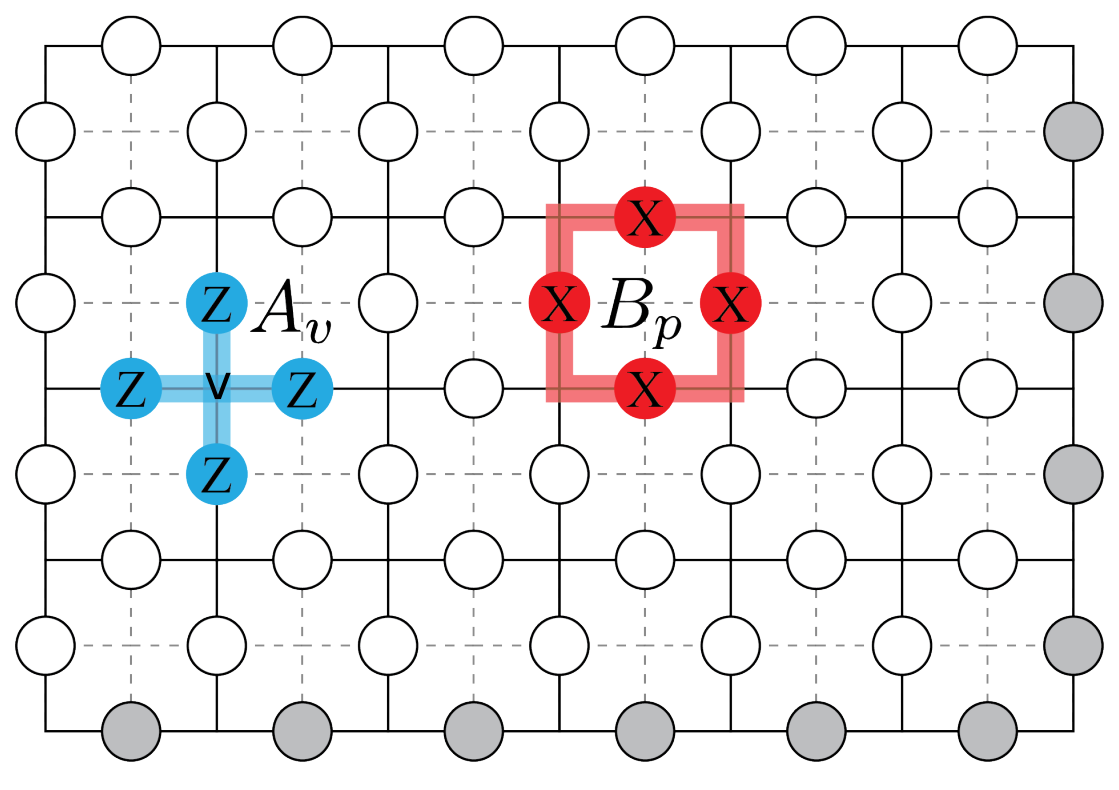
\includegraphics[width=0.7\textwidth]{fig1_intro_toric_codes}\caption{2D Lattice with periodic boundary conditions with . $v$ marks a particular
vertex of the lattice and $p$ marks a particular ``face'' of the
lattice.}
\label{2dlattice}
\end{figure}

Consider a 2D square lattice with periodic boundary conditions\footnote{i.e., a torus}
and single qubit, spin-$\frac{1}{2}$ particles\footnote{e.g., proton, neutron, electron, neutrino}
on each edge (see figure \ref{2dlattice}). Take the standard $X:=\sigma_{x}$
and $Z:=\sigma_{z}$ Pauli operators. Assume the standard convention,
that $\ket{0},\ket{1}$are eigenstates of $Z$, defined such that
\begin{align*}
Z\ket{0} & =+1\ket{0}\\
Z\ket{1} & =-1\ket{1}
\end{align*}
Note that in the $Z$ basis, the $X$ operator acts as a ``spin-flip''
operator:
\begin{align*}
X\ket{0} & =\ket{1}\\
X\ket{1} & =\ket{0}
\end{align*}
Then define ``vertex'' operators $A_{v}$ and ``plaquette'' (face)
operators $B_{p}$:
\begin{align*}
A_{v} & :=\prod_{j\in\text{star}\left(v\right)}Z_{j}\\
B_{p} & :=\prod_{j\in\text{body}\left(p\right)}X_{j}
\end{align*}
where $\text{star}\left(v\right)$ is the set of particles identified
with edges adjacent on the vertex $v$, and $\text{body}\left(p\right)$
is the set of particles identified with the edges surrounding the
plaquette $p$. Note the product here is a tensor product. Then define
the following Hamiltonian
\begin{equation}
H:=-\sum_{v}A_{v}-\sum_{p}B_{p}\label{eq:hamil}
\end{equation}
where $\sum_{v}$ is over all vertices in the lattice and $\sum_{p}$
is over all plaquettes. Recall the Hamiltonian of a system specifies
its total energy.

Facts:
\begin{enumerate}
\item $A_{v}$ and $B_{p}$ are all Hermitian\footnote{$H$ is Hermitian iff $\langle H\psi\vert\psi\rangle=\langle\psi\vert H\psi\rangle=\langle H^{\dagger}\psi\vert\psi\rangle$.
Also sometimes called \emph{self-adjoint.}} and square to the identity\footnote{$A_{v}\cdot A_{v}^{\dagger}\equiv I$}.
Therefore they each (all) have eigenvalues of either $+1$ or $-1$.
\item Each of them commutes with all of the others
\begin{enumerate}
\item $A_{v}$ commutes with $A_{v'}$ because they do not overlap at all
\item $B_{p}$ commutes with $B_{p'}$ overlap on at most one edge and $X_{j}$
always commutes with $X_{j'}$
\item If some $A_{v}$ overlaps with some $B_{p}$ then they overlap on
two edges; the overlapping $Z,X$ (one pair on each edge) each anti-commute
but since there are two such pairs, the effect is cancelled out
\end{enumerate}
\item Therefore, we can measure all the $A_{v}$ and $B_{p}$ simultaneously\footnote{If operators $F$ and $G$ commute, then you can come up with a ``complete''
set of basis states $\ket{f_{n}g_{n}}$ that are eigenstates of both
$F$ and $G$, and thus express any state of the quantum system as
\[
\ket{\Psi}=\sum_{n}\alpha_{n}\ket{f_{n}g_{n}}
\]

Measuring $F$ you will get eigenstate $f_{m}$ with probability $\left|\alpha_{m}^{2}\right|$
and the system will be in eigenstate $\ket{f_{m}g_{m}}$ and similarly
for $G$. Thus, it doesn't matter which order you measure $F,G$ in,
you will get a consistent result. This is the significance of commuting
operators.} and the ground-state energy of $H$ (i.e., the lowest energy state)
will be the product of the $+1$ eigenstates of all of the $A_{v}$
and $B_{p}$\footnote{Since, if you plug $A_{v}\equiv B_{p}\equiv1$ into eqn. (\ref{eq:hamil})
you get the largest negative sum.}
\end{enumerate}
%
All of this should be looking familiar given section \ref{sec:The-stabilizer-formalism}
and it should come as no surprise that $\left\{ A_{v},B_{p}\right\} $
(over all vertices and all faces) comprise a stabilizer subgroup (of
the Pauli group $G_{k}$ on the lattice, where $k$ is the number
of particles captured by the lattice). So what's the dimension of
the code space $T_{S_{k}}$ on this lattice with these stabilizers?
Thinking a little bit imaginatively about $\left\{ A_{v},B_{p}\right\} $
as a set of constraints gives some physical meaning to them: violating
any of the constraints (i.e., a state generating a measurement of
$-1$ from any of the $\left\{ A_{v},B_{p}\right\} $) costs energy
by virtue of the hamiltonian (any $A_{v},B_{p}$ that measures $-1$
will add a positive term to the sum in eqn. (\ref{eq:hamil})). Thus,
the ground-state of the system (i.e., the lowest energy state) should
obey all of the ``constraints'' induced by $\left\{ A_{v},B_{p}\right\} $.
All told the dimension of the code space is \cite{introtoriccode}.

\section{Toric Codes}

But what do the possible legal codes look like? Note (by the just
preceding discussion on satisfying constraints), this is the same
thing as asking what are the ground-states (lowest energy states)
of the system. First, as a kind of warm up, consider only the $A_{v}$
and the system state where each qubit is in the $\ket{0}$ state.
In such a state, all $A_{v}$ would be measured in the $+1$ state
as well. What happens if we apply $X$ to one or two qubits in a row
(i.e., flip two spins)? In this case only vertex operators $A_{v}$
adjacent to those qubits will be affected, through the $Z_{j}$ that
measures $-1$ on the flipped qubit (see figure \ref{spinflips} where
in (a) we show how one such $A_{v}$ is affected). Crucially, notice
that for longer strings of errors ($\geq3$ qubits) it's only the
$A_{v}$ at the ends of the string that will pick up the error. This
ambiguity is what leads to techniques such as minimum weight perfect
matching\cite{https://doi.org/10.48550/arxiv.2105.13082}. What happens
if we flip a sequence of qubits that comprise a ``loop'' on the
lattice? In that case, any $A_{v}$ adjacent to any of the qubits
will have 2 of its 4 $Z_{j}$ measure $-1$ on the flipped qubits
and but since
\[
A_{v}:=Z_{j_{1}}Z_{j_{2}}Z_{j_{3}}Z_{j_{4}}\equiv\left(+1\times+1\right)\times\left(-1\times-1\right)\equiv+1
\]
$A_{v}$ will still be measured in its $+1$ eigenstate. 
\begin{figure}
\centering{}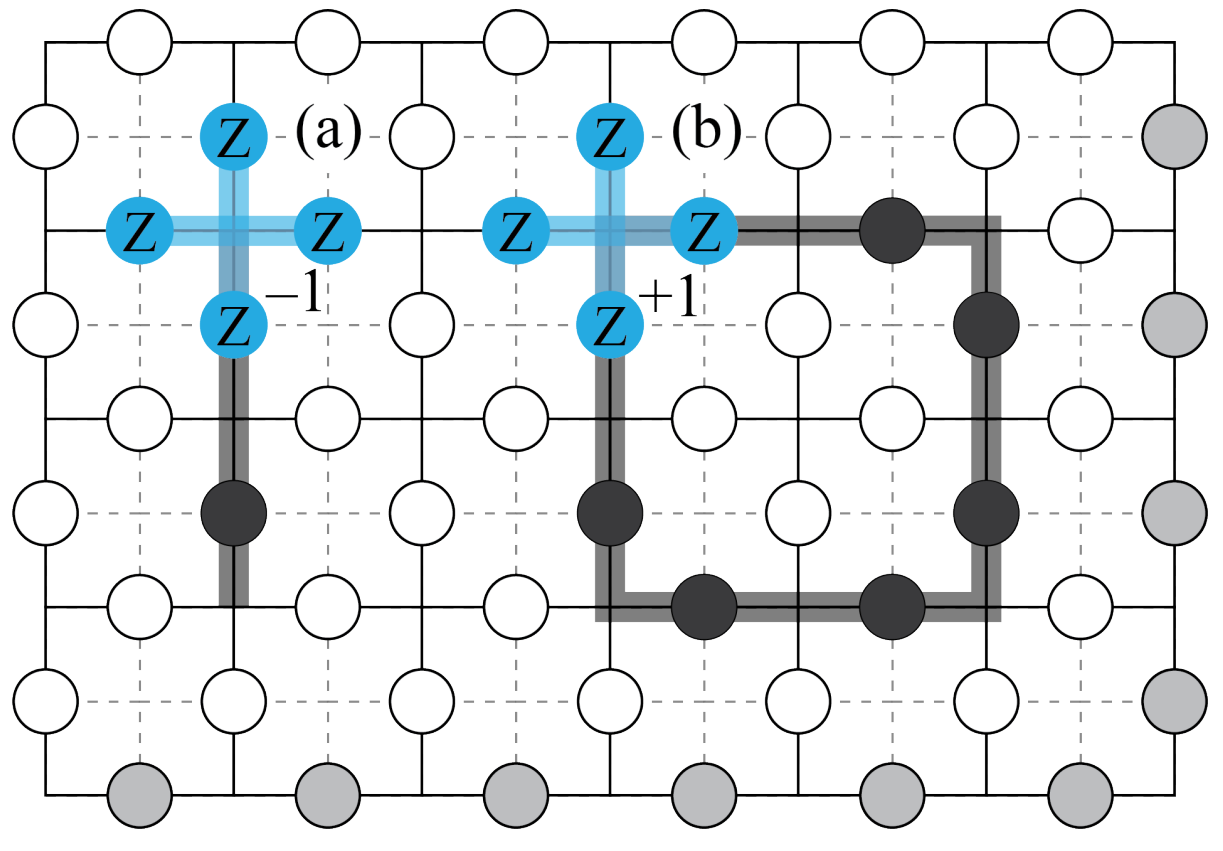
\includegraphics[width=0.7\textwidth]{spinflips}\caption{``Flipped qubits'' are shaded black. In (a) we consider a short
string of flipped qubits and in (b) we consider a loop of flipped
qubits.}
\label{spinflips}
\end{figure}
Indeed there are many, many such possible states (with some number
of non-flipped qubits but also loops of flipped qubits). This is called
\emph{degeneracy}, when lots of distinct physical states are measured
to have the same energy. In particular (you'll see why in a second),
if we only measure $A_{v}$, loops that go over the edge and back
aroud (i.e., all the way around the torus), will also be indistringuishable
from the groundstate.

Recall that what we're trying to accomplish in constructing error
correcting codes is to discover particular states of our quantum system
(in this case, a lattice of spin-$\frac{1}{2}$ particles) can be
in that can be distinguished between using non-destructive measurements
(in this case, using stabilizers). Therefore such degeneracy is problematic.
The resolution is to apply the $B_{p}$, i.e., measure $B_{p}$ \emph{as
well as} the $A_{v}$. What does this accomplish? Well looking at
figure \ref{spinflipswithbp}, it seems like not much, but in fact
we can use the $B_{p}$ to completely eliminate any loop of spin flips,
by applying the $B_{p}$ adjacent to the interior edge of the loop
(see figure \ref{spinflipswithbp-1}). 
\begin{figure}
\centering{}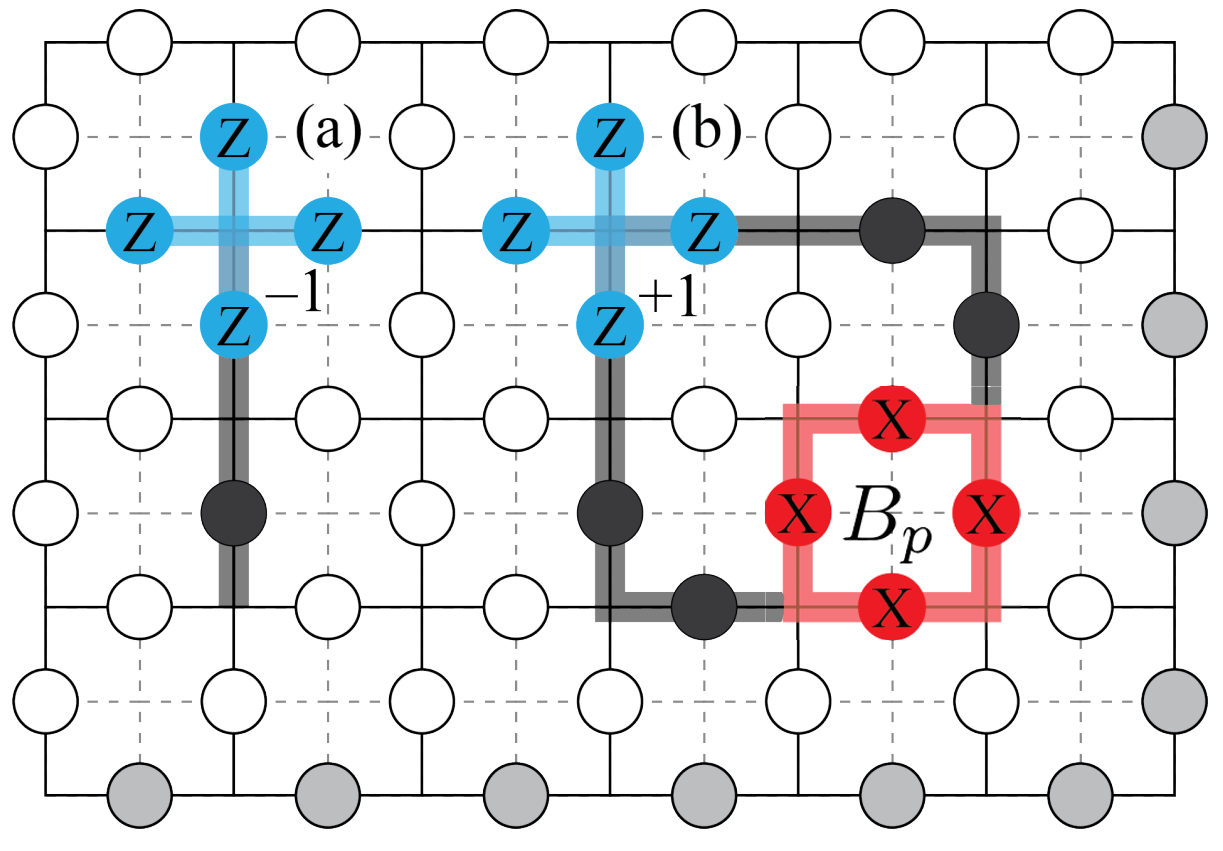
\includegraphics[width=0.7\textwidth]{spinflipswithbp}\caption{Both $A_{v}$ and $B_{p}$ being measured.}
\label{spinflipswithbp}
\end{figure}
\begin{figure}
\centering{}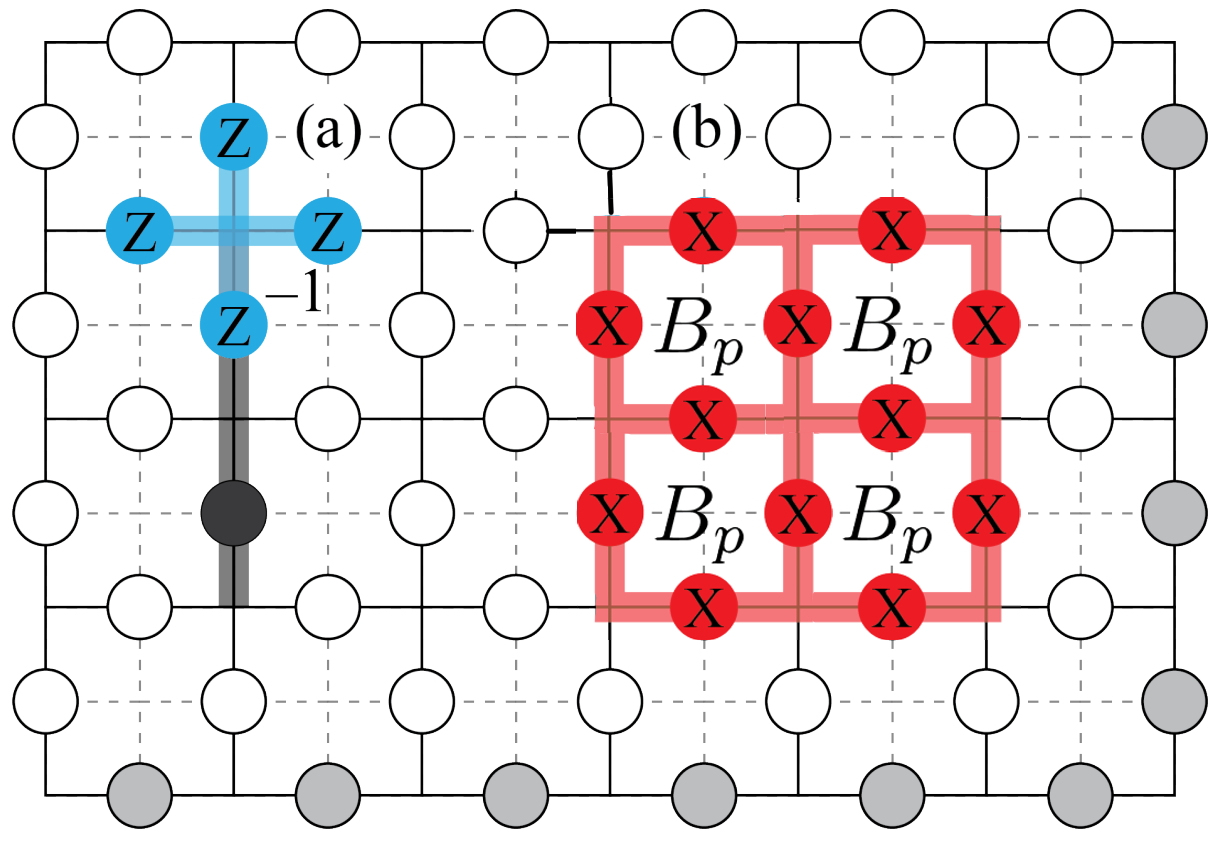
\includegraphics[width=0.7\textwidth]{spinflipswithbplooperase}\caption{Using $B_{p}$ to collapse the loop in fig. \ref{spinflipswithbp}
- notice that the $X$ operators flip the flipped spins ``back to
normal'' \emph{and} cancel each other out (on the interior).}
\label{spinflipswithbp-1}
\end{figure}
But measuring $B_{p}$ along with $A_{v}$ doesn't resolve all ambiguities;
consider a loop of flipped spins that extends all the way around the
edge of the lattice (i.e., wraps around an axis of the torus). Applying
$B_{p}$ to each particle along such a loop would simply shift the
loop laterally. \textbf{Thus, we have found the set of undetectable
errors for this coding scheme}, i.e., the set $\left\{ \bar{X_{1}},\bar{X_{2}},\bar{Z_{1}},\bar{Z_{2}}\right\} $
of \emph{Toric codes} (see figure \ref{spinflipswithbp-1-1}). The
fact that there are only four such codes is intimately related to
the dimension\cite{toriccodes} of the stabilizer group (which we
earlier computed to be 4).
\begin{figure}
\centering{}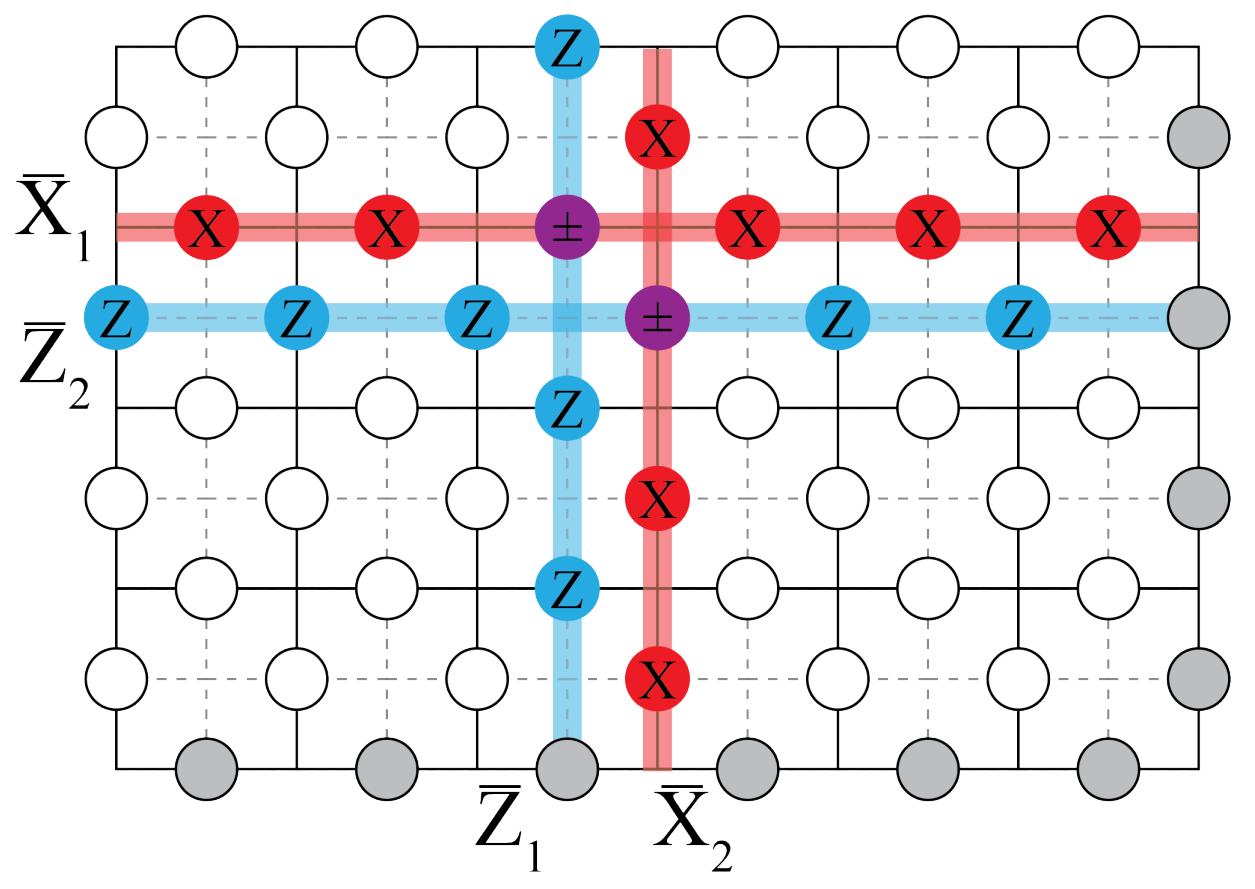
\includegraphics[width=0.7\textwidth]{toriclogicbits}\caption{The fourse possible logical operators $\bar{X_{1}}$, $\bar{X_{2}}$,
$\bar{Z_{1}}$, $\bar{Z_{2}}$.}
\label{spinflipswithbp-1-1}
\end{figure}

\bibliographystyle{plain}
\bibliography{main}

\end{document}
